\documentclass[10pt,twocolumn]{article}
\usepackage[letterpaper,top=0.75in,bottom=0.75in,left=0.75in,right=0.75in,columnsep=0.25in]{geometry}
\usepackage{times}
\usepackage{graphicx}
\usepackage{booktabs}
\usepackage{amsmath}
\usepackage{url}
\usepackage{microtype}
\usepackage{caption}
\usepackage{enumitem}
\usepackage{float}
\captionsetup{font=footnotesize,labelfont=bf}
\setlength{\parindent}{1em}
\setlength{\parskip}{0pt}
\setlist{nosep,leftmargin=*}

\title{SLO-Aware Recovery-Stage-Adaptive Control for Kubernetes Microservices under Dynamic Workloads}
\author{Adnan Yunus Mohammed\\DePaul University\\NET 470 Cloud Networking\\Prof. Nazli Siasi}
\date{}

\begin{document}
\maketitle

\begin{abstract}
This paper evaluates SLO-aware recovery-stage-adaptive control for a Kubernetes microservice application across five increasing workload levels: 5, 10, 15, 20, and 25 requests/s. The balanced randomized experiment compares five configurations (C1--C5) under the same phase durations, application, resource limits, and 123.472-ms latency SLO. Five blocks per workload-treatment cell produced 125 scientifically admissible episodes and 581,250 scheduled requests; 581,240 completed and 10 returned errors. Outcomes comprised 72 episodes without a qualifying breach, 32 observed recoveries, and 21 recoveries right-censored at 300 s. At 20 requests/s, tuned static HPA C2 achieved conditional KM RMST(300) of 203.666 s, whereas the proposed C5 controller required 253.595 s, increased mean SLO-violation duration by 42 s, and consumed 241.574 additional replica-seconds. At 25 requests/s, C2 recovered in three of five episodes, while all five C5 episodes were censored. Stage analysis explains the result: T7--T8 application stabilization dominated the measured recovery path, while C5 targeted the earlier T1--T2 HPA-response stage and became redundant after the five-replica ceiling was reached. Thus, C5 was reproducible and safely restored the HPA, but its performance superiority was not supported. The contribution is a controlled five-level evaluation that exposes when an interpretable adaptive action helps, adds cost, or misses the dominant recovery stage.
\end{abstract}

\noindent\textbf{Index Terms---}Kubernetes, HPA, microservices, SLO, recovery time, right censoring, stage-aware control, RMST.

\section{Introduction}
Horizontal Pod Autoscaling (HPA) changes desired capacity in response to resource pressure, but a scaling decision is not equivalent to stable application recovery. Kubernetes computes resource utilization relative to configured requests and uses this signal to recommend replicas~\cite{k8shpa}. A replica must still be scheduled, started, become ready, receive traffic, and contribute to sustained SLO compliance. Consequently, a controller that accelerates an early infrastructure stage may not reduce end-to-end recovery if a later application stage dominates.

This project measures the complete T0--T8 path from workload transition and HPA response through pod lifecycle, traffic activation, and stable latency. It evaluates whether a bounded recovery-stage-aware controller (C5) improves recovery over static and guarded alternatives. The final study responds to three questions: (Q1) how recovery changes from normal operation to overload; (Q2) whether C5 reduces recovery time and SLO violations relative to tuned HPA C2; and (Q3) whether any benefit is achieved without excessive resource cost.

Prior systems motivate bottleneck-aware scaling, fine-grained diagnosis, and explicit SLO feedback~\cite{pbscaler,firm,autothrottle}. Our narrower contribution is an auditable controlled experiment: five workloads, five treatments, identical constraints, explicit censoring, block-level replication, and exact restoration. The results are deliberately reported without smoothing or replacing unsuccessful recovery outcomes.

\begin{table}[t]
\centering
\caption{Position Relative to Representative Prior Work}
\label{tab:related}
\resizebox{\columnwidth}{!}{%
\begin{tabular}{lll}
\toprule
Work & Primary focus & Distinction here\\
\midrule
PBScaler & Bottleneck-aware scaling & Explicit T0--T8 timing\\
FIRM & Fine-grained diagnosis & Bounded action/rollback\\
Autothrottle & Bi-level SLO control & Auditable stage trigger\\
\bottomrule
\end{tabular}}
\end{table}

\section{System and Recovery Model}
\subsection{Application and Fixed Protocol}
The application contains Ingestion, Processing, and Results services. Processing performs deterministic CPU-bound work and is the HPA target. Every episode uses the same four phase durations: 60 s low precondition, 180 s challenge, 300 s low recovery, and 30 s post-observation. Only the challenge rate changes across 5, 10, 15, 20, and 25 requests/s. Therefore, the total scheduled requests per episode are 2,850, 3,750, 4,650, 5,550, and 6,450, respectively. The latency SLO is 123.472 ms on emitted 15-s windows. The processing HPA uses one to five replicas, with C2 tuned to a 55\% CPU target.

\begin{table}[t]
\centering
\caption{Five-Level Frozen Experimental Design}
\label{tab:design}
\begin{tabular}{lrrrrr}
\toprule
Challenge rate (RPS) & 5 & 10 & 15 & 20 & 25\\
\midrule
Requests/episode & 2850 & 3750 & 4650 & 5550 & 6450\\
Cells (C1--C5) & 5 & 5 & 5 & 5 & 5\\
Episodes & 25 & 25 & 25 & 25 & 25\\
\bottomrule
\end{tabular}
\end{table}

\subsection{T0--T8 and Stable Recovery}
The nine boundaries are: T0 workload-path origin; T1 first positive metric/HPA observation; T2 native HPA scaling action; T3 pod creation; T4 scheduling; T5 container start; T6 readiness; T7 traffic activation and first bound request; and T8 application stabilization. For observed boundaries,
\begin{equation}
T_8-T_0=\sum_{i=0}^{7}(T_{i+1}-T_i).
\end{equation}
A breach boundary $T_B$ is declared by the frozen consecutive-bad-window rule. $T_R$ is the first boundary at which consecutive windows confirm sustained SLO compliance. If recovery is not observed within 300 s, the outcome is right-censored:
\begin{equation}
Y_i=\min(T_R-T_B,300),\quad \delta_i=I(T_R-T_B\leq300).
\end{equation}
A no-breach episode has no recovery duration and is not encoded as zero. Conditional Kaplan--Meier restricted mean survival time, RMST(300), summarizes breach episodes while retaining censored outcomes.

\begin{table}[t]
\centering
\caption{Operational T0--T8 Recovery Boundaries}
\label{tab:boundaries}
\resizebox{\columnwidth}{!}{%
\begin{tabular}{ll}
\toprule
Event & Operational meaning\\
\midrule
T0 & Workload-path origin\\
T1 & First positive metric/HPA observation\\
T2 & Native HPA scaling action\\
T3 & Pod creation\\
T4 & Pod scheduled\\
T5 & Container started\\
T6 & Pod ready\\
T7 & Traffic activation and first bound request\\
T8 & Stable application-level SLO recovery\\
\bottomrule
\end{tabular}}
\end{table}

\section{Controllers}
Table~\ref{tab:treatments} separates static scaling, diagnosis, and adaptation. C1 and C2 are static HPA baselines. C3 observes and diagnoses without changing HPA. C4 applies a guarded bounded adaptation. C5 is the proposed T1--T2 recovery-stage-aware controller.

\begin{table}[t]
\centering
\caption{Compared Configurations}
\label{tab:treatments}
\begin{tabular}{lll}
\toprule
ID & Role & HPA modification\\
\midrule
C1 & Reference static HPA & None\\
C2 & Tuned static HPA (55\%) & None\\
C3 & Diagnosis only & None\\
C4 & Guarded adaptation & Bounded action\\
C5 & T1--T2 stage-aware control & One floor action\\
\bottomrule
\end{tabular}
\end{table}

C5 requires CPU support, increased desired replicas, two consecutive positive observations, an exceeded calibrated T1--T2 budget, and positive utility. Candidate minimum-replica targets $n\in\{2,3,4,5\}$ are scored by
\begin{equation}
U(n)=\frac{\mathrm{CPU}}{55}\left(1-\frac{1}{n}\right)-0.15(n-1).
\end{equation}
At most one minimum-floor action is authorized. The original HPA specification is restored at the low-recovery boundary and again unconditionally in a \texttt{finally} path. This bounded rule is interpretable, but it cannot exceed the five-replica ceiling and acts directly on T1--T2 rather than T7--T8.

\begin{table}[t]
\centering
\caption{C5 Production Decision and Restoration Rules}
\label{tab:rules}
\resizebox{\columnwidth}{!}{%
\begin{tabular}{ll}
\toprule
Observed condition & Controller decision\\
\midrule
Outside high-challenge phase & HOLD\\
CPU support absent or desired replicas $\leq1$ & HOLD\\
First positive observation only & HOLD pending confirmation\\
Elapsed time below calibrated T1--T2 budget & HOLD\\
Maximum candidate utility below threshold & HOLD\\
Qualified trigger with no prior action & Set selected HPA minimum\\
Low-recovery boundary or completion & Restore exact original HPA\\
\bottomrule
\end{tabular}}
\end{table}

\section{Experimental and Statistical Method}
Five randomized blocks were executed at each workload. Every block contained C1--C5 once, yielding five observations per cell and 125 selected episodes. Workload duration, application version, SLO, HPA limits, and resource constraints were held fixed across treatments. The earliest technically valid attempt was selected; four excluded attempts were preserved with their failure records. Every selected episode restored the original HPA configuration.

Recovery analysis is conditional on a qualifying breach. Recovered episodes are events and unsuccessful recoveries are censored at 300 s. No-breach episodes are reported separately. SLO-violation duration and replica-seconds include all five episodes in each cell. Error bars are deterministic block-bootstrap 95\% percentile intervals over the five experimental blocks. Request rows are observations within an episode, not independent treatment replicates.

\section{Results}
The experiment scheduled 581,250 requests; 581,240 completed and 10 returned errors (99.998\% completion). Across 125 episodes, 72 had no qualifying breach, 32 recovered within 300 s, and 21 were right-censored. At 5 and 10 RPS the application usually remained within the SLO. At 15 RPS breaches began to appear. All treatments experienced breaches at 20 RPS, and overload at 25 RPS produced 18 censored outcomes across 25 episodes.

\begin{figure*}[t]
\centering
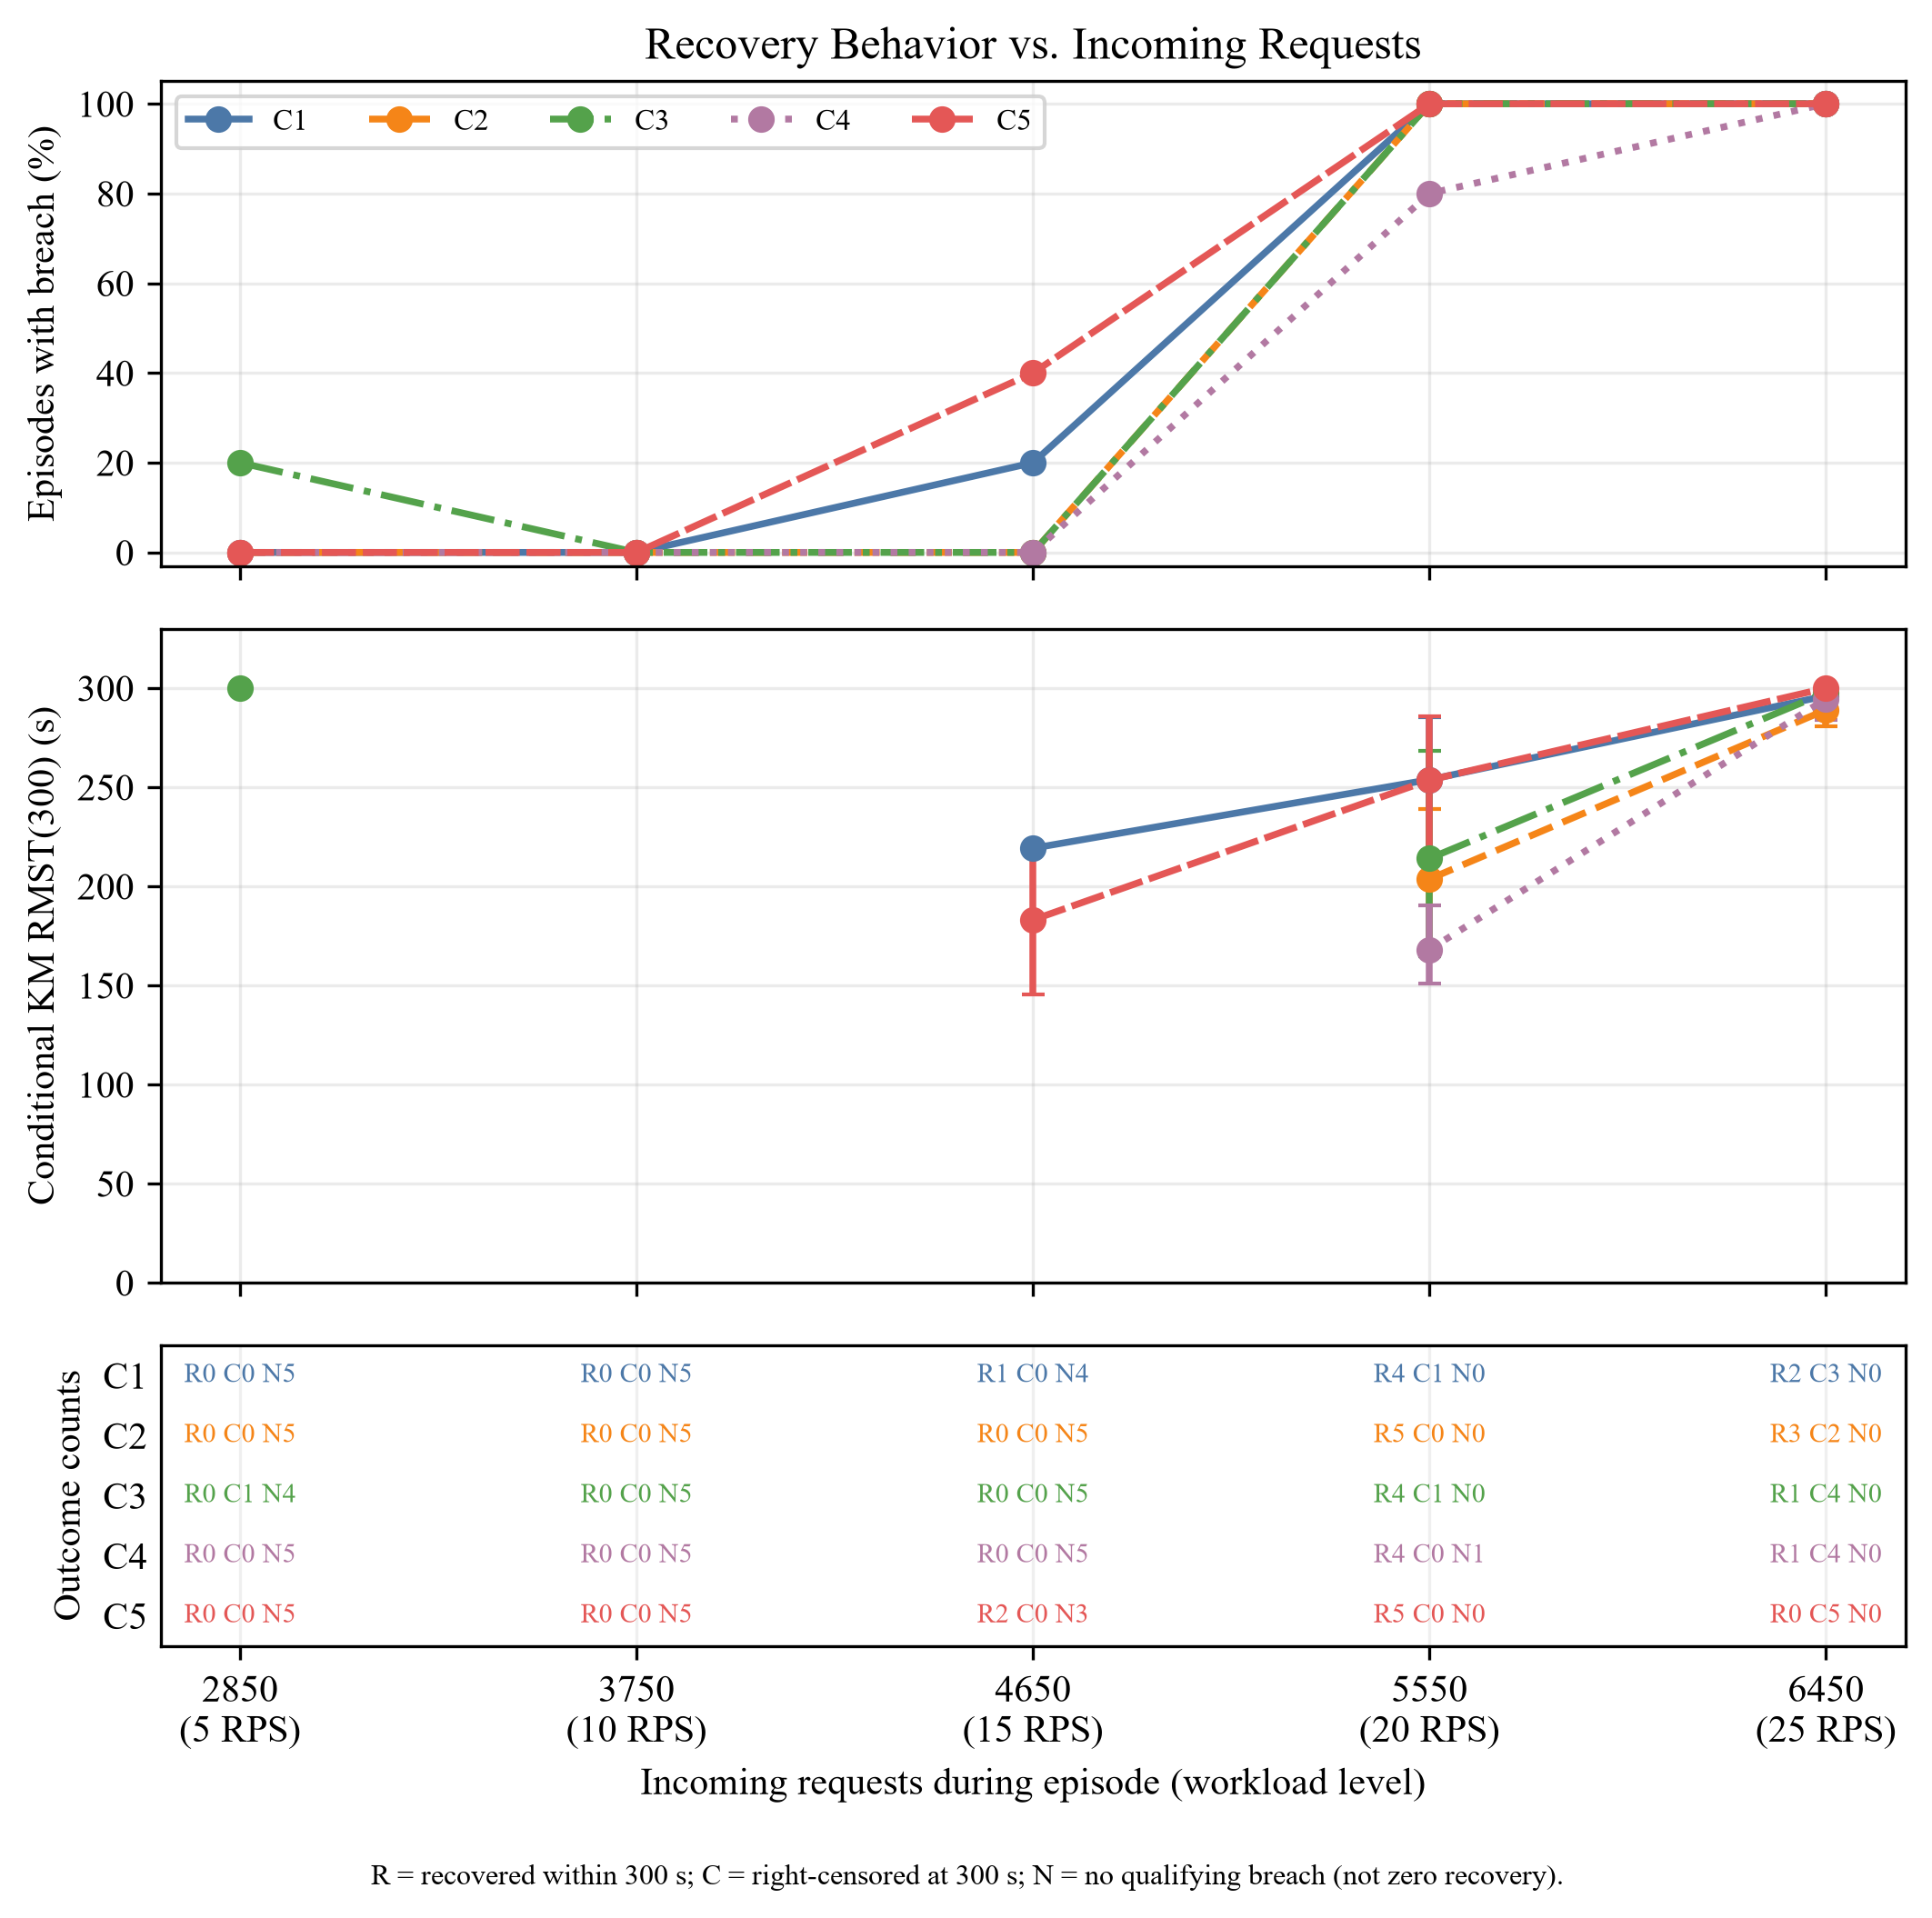
\includegraphics[width=0.96\textwidth]{figures/figure1_recovery_vs_requests.png}
\caption{Recovery behavior versus incoming requests. The top panel reports breach incidence. The middle panel reports conditional KM RMST(300) with block-bootstrap 95\% intervals. The bottom panel distinguishes recovered (R), right-censored (C), and no-breach (N) episodes. No-breach episodes are not encoded as zero recovery.}
\label{fig:recovery}
\end{figure*}

\subsection{Recovery Time and Censoring}
Figure~\ref{fig:recovery} shows nonlinear degradation near saturation. At 20 RPS all five C2 and C5 episodes recovered, but C2 RMST(300) was 203.666 s (95\% CI 169.607--239.090), compared with 253.595 s (212.018--285.782) for C5. C5 was therefore 49.929 s, or 24.5\%, slower. C4 had the lowest 20-RPS point estimate, 168.059 s (150.735--190.342), but its five-block sample is too small for a universal superiority claim.

At 25 RPS, C2 recovered in three episodes and was censored in two, giving RMST(300)=289.024 s (280.706--297.288). C5 recovered in none and was censored in all five, giving RMST(300)=300 s. C5 did not reduce recovery near saturation or overload. The isolated C3 censoring at 5 RPS is retained as observed variability rather than removed as an inconvenient point.

\begin{table}[t]
\centering
\caption{C5 Relative to C2 at High Load}
\label{tab:c5c2}
\begin{tabular}{lrr}
\toprule
Metric (C5$-$C2) & 20 RPS & 25 RPS\\
\midrule
RMST(300), s & +49.929 & +10.976\\
SLO violation, s & +42.000 & +24.000\\
Replica-seconds & +241.574 & +26.630\\
Mean CPU, points & +0.536 & +5.915\\
T7--T8, s & +20.772 & +1.809\\
\bottomrule
\end{tabular}
\end{table}

\subsection{SLO Violations}
Figure~\ref{fig:slo} compares violation duration across all episodes. At 20 RPS, mean violation duration was 96 s for C2, 60 s for C4, and 138 s for C5. Thus C5 added 42 s relative to C2 and 78 s relative to C4. At 25 RPS, C2 averaged 168 s and C5 192 s. The curves show the expected saturation effect: violation duration grows sharply between 15 and 20 RPS and remains high at 25 RPS. C5 did not maintain more stable performance as load increased.

\begin{figure}[H]
\centering
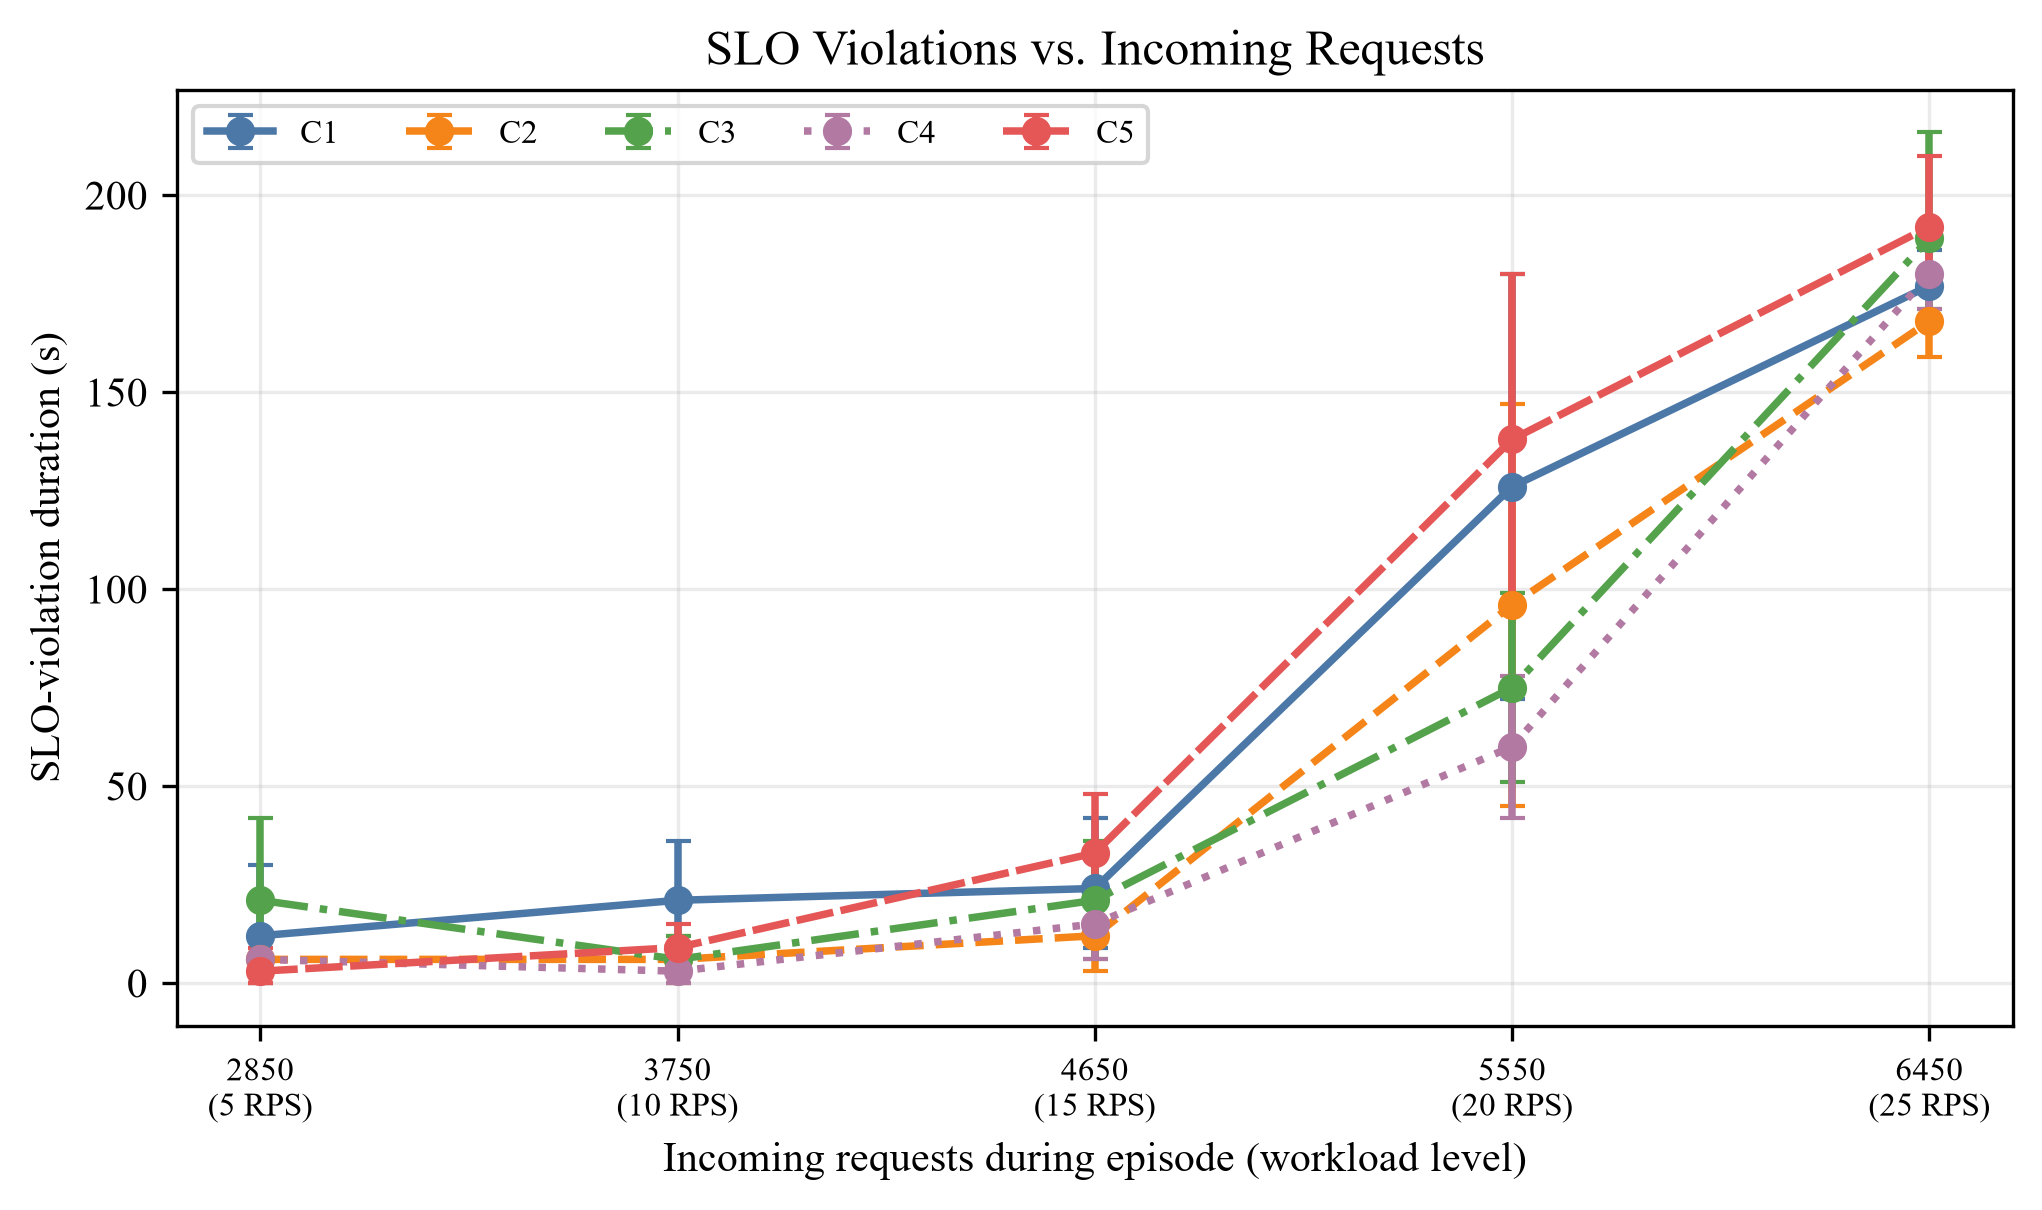
\includegraphics[width=\columnwidth]{figures/figure2_slo_violations_vs_requests.png}
\caption{Mean SLO-violation duration versus incoming requests with block-bootstrap 95\% intervals. Lines connect observed workload-level estimates only; no smoothing is applied.}
\label{fig:slo}
\end{figure}

\subsection{Resource Cost}
Figure~\ref{fig:resource} reports replica-seconds under identical one-to-five-replica limits. At 10 RPS, no C2 or C5 episode breached, yet C5 acted in all five episodes, increased mean peak desired replicas from 2 to 3, and consumed 1,435.926 replica-seconds versus 1,038.423 for C2---a 38.3\% increase without recovery benefit. At 20 RPS, C5 consumed 2,259.779 replica-seconds, 241.574 more than C2. At 25 RPS all methods approached the replica ceiling; C5 still used 26.630 more replica-seconds and 5.915 additional mean CPU percentage points than C2.

\begin{figure}[H]
\centering
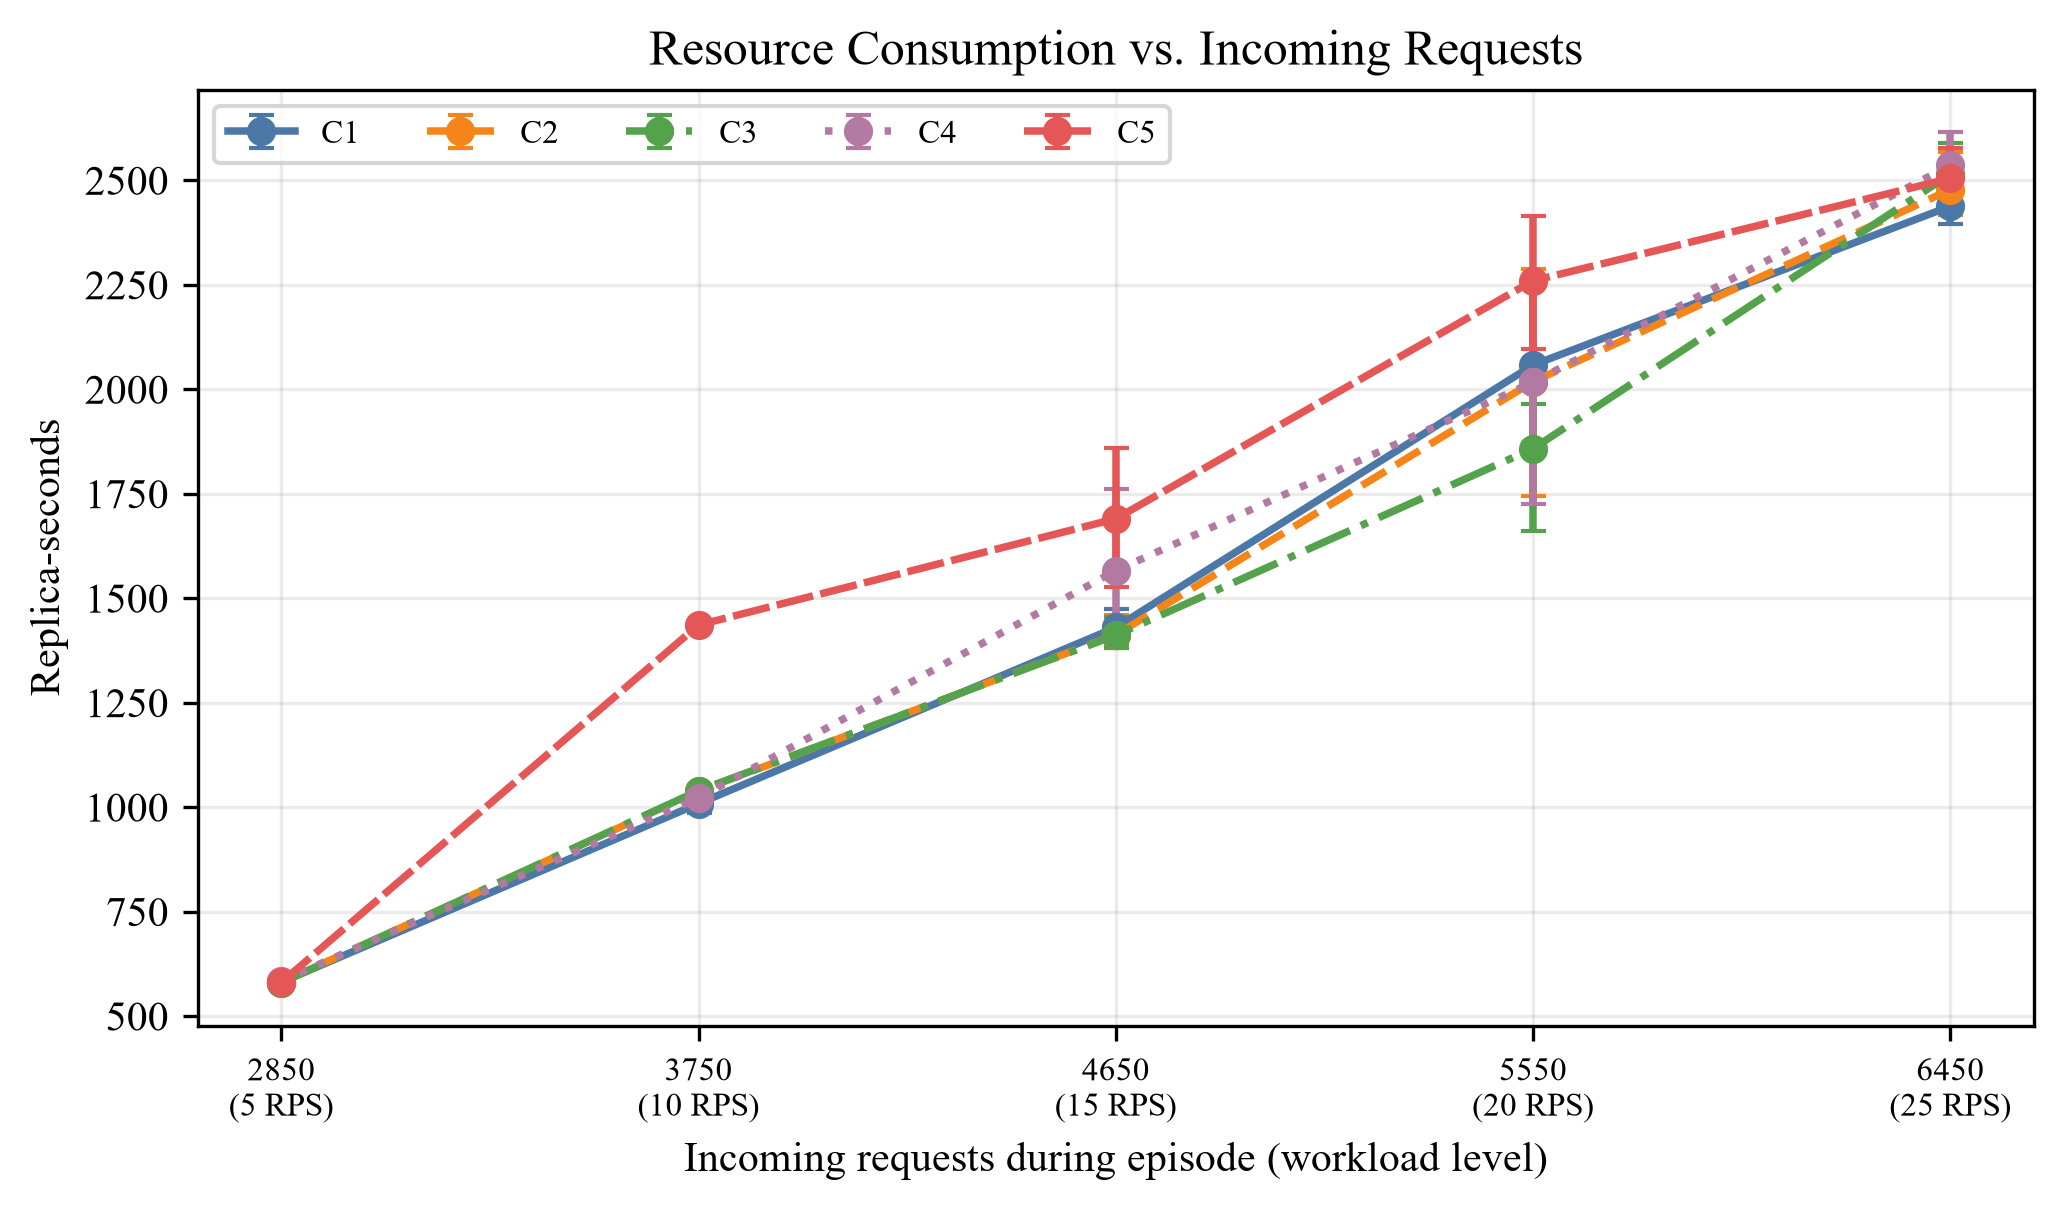
\includegraphics[width=\columnwidth]{figures/figure3_resource_vs_requests.png}
\caption{Mean replica-seconds versus incoming requests with block-bootstrap 95\% intervals under identical resource constraints.}
\label{fig:resource}
\end{figure}

\subsection{Why C5 Did Not Improve Recovery}
The intervention and stage measurements explain the outcome. C5 authorized one action in every episode from 10 through 25 RPS. At 20 RPS, its mean peak desired and ready replicas were both 4.6, compared with 4.2 for C2; however, mean T7--T8 was 86.835 s for C5 and 66.063 s for C2. T4--T5 was only 1.6 s and T6--T7 only 0.923 s for C5. At 25 RPS, desired and ready replicas were already 5.0 for every treatment. Raising the HPA minimum could not create capacity beyond the configured maximum.

\begin{table*}[t]
\centering
\caption{Controller Action and Recovery-Stage Evidence at High Load}
\label{tab:mechanism}
\resizebox{\textwidth}{!}{%
\begin{tabular}{llrrrrrr}
\toprule
RPS & Treatment & Action episodes & Peak desired & Peak ready & Mean CPU (\%) & T4--T5 (s) & T7--T8 (s)\\
\midrule
20 & C2 & 0/5 & 4.2 & 4.2 & 51.186 & 1.4 & 66.063\\
20 & C4 & 4/5 & 4.2 & 4.2 & 45.464 & 1.2 & 39.142\\
20 & C5 & 5/5 & 4.6 & 4.6 & 51.723 & 1.6 & 86.835\\
25 & C2 & 0/5 & 5.0 & 5.0 & 66.679 & 1.6 & 175.705\\
25 & C4 & 5/5 & 5.0 & 5.0 & 62.857 & 2.0 & 187.349\\
25 & C5 & 5/5 & 5.0 & 5.0 & 72.593 & 2.2 & 177.513\\
\bottomrule
\end{tabular}}
\end{table*}

Across treatments, T7--T8 increased from roughly 8--9 s at 10 RPS to 176--187 s at 25 RPS. The dominant delay was therefore post-readiness application stabilization, not HPA decision, scheduling, or readiness. C5's T1--T2 action was temporally and causally misaligned with the measured bottleneck. C4's selective behavior---actions in four of five 20-RPS episodes instead of unconditional C5 action---is a promising direction, but at 25 RPS C4 also had four censored episodes. The evidence supports refinement, not a claim that guarded adaptation always wins.

\section{Discussion and Limitations}
The main hypothesis was not supported: the evaluated C5 rule did not recover faster than tuned HPA C2. This negative result is technically informative. It shows that stage awareness must connect diagnosis to an action that can affect the dominant controllable stage. A bounded C5-R follow-up could add queue, concurrency, or application-stabilization control for T7--T8 and suppress action when no qualifying breach exists. Such a controller must be calibrated and evaluated separately; it must not replace or rewrite the frozen primary dataset.

The study uses one Windows-hosted Minikube node, one service topology, five blocks per cell, one latency SLO, and one maximum-replica setting. Confidence intervals are consequently wide in some cells, and overlapping intervals do not establish equivalence. T1 is interval-censored and native events have finite timestamp resolution. Results may change with other burst shapes, service graphs, resource requests, or cluster sizes. Four technically invalid attempts were excluded by a predeclared qualification rule and preserved in the evidence package. The selected 125 episodes had no timeout, duplicate design cell, or failed HPA restoration.

The optional throughput figure was omitted because achieved throughput followed the offered rates and only 10 of 581,250 requests failed; it would add little beyond the three requested performance figures. Completion is reported numerically to avoid hiding these errors while preserving space for recovery, SLO, and resource evidence.

\clearpage
\section{Conclusion}
This work completes a balanced five-level C1--C5 evaluation with 125 scientifically admissible episodes and explicit right censoring. C5 was implemented, executed, and safely restored, but it did not improve recovery over C2. At 20 RPS it was 24.5\% slower, produced longer SLO violations, and consumed more replica-seconds. At 25 RPS every C5 episode was censored while C2 recovered in three of five. The dominant T7--T8 stabilization stage and the five-replica ceiling explain why the early HPA-floor intervention did not translate into end-to-end benefit. The central engineering conclusion is alignment: adaptive recovery requires an action that targets the dominant stage and remains useful under the active capacity constraint.

\section*{Data and Reproducibility}
The repository contains the controller and runner, frozen 125-row primary dataset, three figure-generation scripts, statistical tables, technical-exclusion records, and SHA-256 manifests. The primary dataset SHA-256 is \texttt{B7939B0FFE443AD76AC5ECE693CDFC03015C735895D27835E2DE2AF1A87781BD}. Repository: \url{https://github.com/mdadnan-dev/slo-aware-kubernetes-recovery}.

\begin{thebibliography}{4}
\bibitem{k8shpa} Kubernetes, ``Horizontal Pod Autoscaling,'' Kubernetes Documentation, accessed Nov. 7, 2026. [Online]. Available: \url{https://kubernetes.io/docs/concepts/workloads/autoscaling/horizontal-pod-autoscale/}
\bibitem{pbscaler} S. Xie, J. Wang, B. Li, Z. Zhang, D. Li, and P. C. K. Hung, ``PBScaler: A Bottleneck-Aware Autoscaling Framework for Microservice-Based Applications,'' \emph{IEEE Trans. Services Computing}, vol. 17, no. 2, pp. 604--616, 2024, doi: 10.1109/TSC.2024.3376202.
\bibitem{firm} H. Qiu, S. S. Banerjee, S. Jha, Z. T. Kalbarczyk, and R. K. Iyer, ``FIRM: An Intelligent Fine-Grained Resource Management Framework for SLO-Oriented Microservices,'' in \emph{Proc. 14th USENIX OSDI}, 2020, pp. 805--825.
\bibitem{autothrottle} Z. Wang, P. Li, C.-J. M. Liang, F. Wu, and F. Y. Yan, ``Autothrottle: A Practical Bi-Level Approach to Resource Management for SLO-Targeted Microservices,'' in \emph{Proc. 21st USENIX NSDI}, 2024, pp. 149--165.
\end{thebibliography}

\end{document}
